\chapter{Release 1}

\begin{spacing}{1.2}
\minitoc
\thispagestyle{MyStyle}
\end{spacing}
\newpage

\section*{INTRODUCTION}
\noindent Dans ce chapitre, nous présentons la première release de l'application « Prévention Plus » qui se compose de deux sprints distincts. Cette release établit les fondations du système avec la gestion de l'authentification, l'inscription des entreprises, le traitement des requêtes d'inscription et la gestion des profils utilisateur dans le premier sprint. Le second sprint abordera les fonctionnalités de gestion des utilisateurs, entreprises, notifications et abonnements.

\section{Sprint 1 : Authentification, inscription, requêtes d'inscription et profils}

\subsection{Spécifications fonctionnelles}
\noindent Ce sprint représente la première phase de notre projet, établissant les mécanismes d'accès et de gestion des comptes utilisateurs.

\subsubsection{Backlog du Sprint 1}
\noindent Le sprint backlog est constitué à partir du backlog produit présenté au chapitre 2. Pour ce premier sprint, nous avons sélectionné les quatre user stories fondamentales présentées dans le tableau 4.1.

\begin{longtable}{|>{\raggedright\arraybackslash}p{4cm}|>{\raggedright\arraybackslash}p{7cm}|>{\raggedright\arraybackslash}p{2cm}|}
\caption{Backlog du sprint 1}
\label{tab:sprint1_backlog}\\
\hline
Histoire utilisateur & Description & Priorité \\
\hline
\endfirsthead
\multicolumn{3}{c}{\tablename\ \thetable\ -- suite} \\
\hline
Histoire utilisateur & Description & Priorité \\
\hline
\endhead
Authentification & En tant que Super Admin, Admin ou Auditeur, je veux m'authentifier avec une adresse e-mail unique pour accéder à mes fonctionnalités & Élevée \\
\hline
Inscription & En tant qu'Admin, je veux m'inscrire et créer le compte de mon entreprise simultanément pour accéder au système & Élevée \\
\hline
Gestion des demandes d'inscription & En tant que Super Admin, je veux accepter ou rejeter les demandes d'inscription pour contrôler l'accès au système & Élevée \\
\hline
Consultation du profil & En tant qu'utilisateur, je veux consulter mon profil pour accéder à mes informations personnelles & Moyenne \\
\hline
Modification du profil & En tant qu'utilisateur, je veux modifier mon profil pour mettre à jour mes informations personnelles & Moyenne \\
\hline
\end{longtable}

\subsubsection{Diagramme de cas d'utilisation détaillé de l'authentification}
\noindent La figure 4.1 présente le diagramme de cas d'utilisation détaillé pour l'authentification, illustrant les interactions entre les différents acteurs et le système.

\begin{figure}[H]
    \centering
    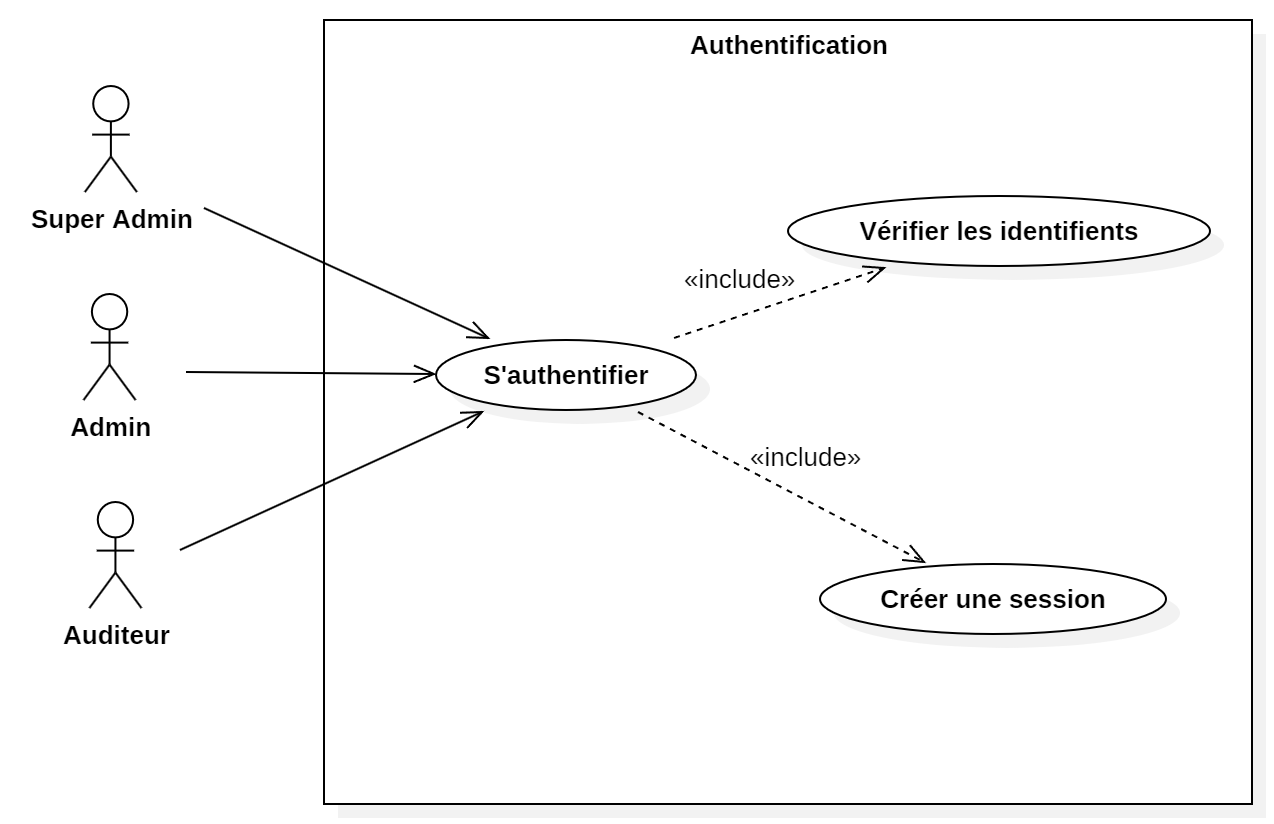
\includegraphics[width=10cm,height=6cm]{images/authuc.png}
    \caption{Diagramme de cas d'utilisation - Authentification}
\end{figure}

\begin{longtable}{|>{\raggedright\arraybackslash}p{4cm}|>{\raggedright\arraybackslash}p{9cm}|}
\caption{Description textuelle du cas d'utilisation - Authentification}
\label{tab:auth_usecase} \\
\hline
\textbf{Cas d'utilisation} & \textbf{S'authentifier} \\
\hline
\textbf{Acteur} & Super Admin, Admin, Auditeur \\
\hline
\textbf{Précondition} & Avoir un compte vérifié et approuvé \\
\hline
\textbf{Postcondition} & L'utilisateur est connecté et redirigé vers son tableau de bord \\
\hline
\textbf{Scénario nominal} & 
1. L'utilisateur accède à la page d'authentification \\
& 2. Le système affiche le formulaire de connexion \\
& 3. L'utilisateur saisit son email et son mot de passe \\
& 4. L'utilisateur clique sur "Connexion" \\
& 5. Le système valide les identifiants \\
& 6. Le système vérifie que l'email est vérifié \\
& 7. Le système vérifie le statut du compte \\
& 8. Le système crée une session utilisateur \\
& 9. Le système redirige vers le tableau de bord approprié \\
\hline
\textbf{Scénario alternatif} & 
- Email ou mot de passe incorrect : affichage d'un message d'erreur \\
& - Email non vérifié : demande de vérification \\
& - Compte en attente d'approbation : message d'attente \\
& - Entreprise non approuvée : message d'attente d'approbation \\
\hline
\end{longtable}

\subsubsection{Diagramme de cas d'utilisation détaillé de l'inscription}
\noindent La figure 4.2 présente le diagramme de cas d'utilisation pour l'inscription d'une entreprise et la création simultanée du compte administrateur.

\begin{figure}[H]
    \centering
    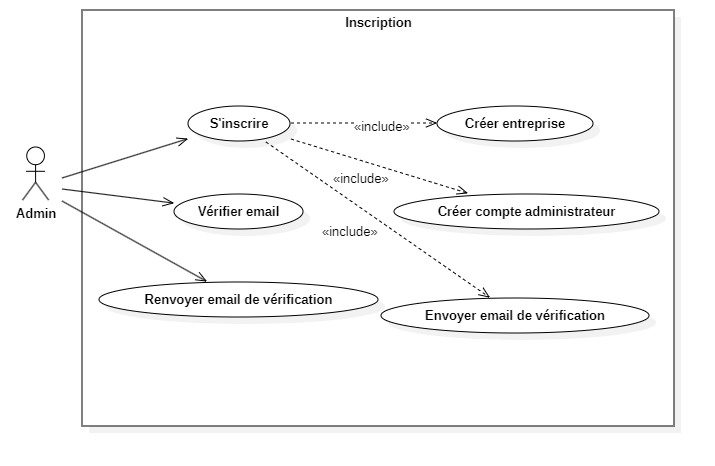
\includegraphics[width=12cm,height=8cm]{images/inscriptionuc.png}
    \caption{Diagramme de cas d'utilisation - Inscription}
\end{figure}

\begin{longtable}{|>{\raggedright\arraybackslash}p{4cm}|>{\raggedright\arraybackslash}p{9cm}|}
\caption{Description textuelle du cas d'utilisation - Inscription}
\label{tab:signup_usecase} \\
\hline
\textbf{Cas d'utilisation} & \textbf{S'inscrire} \\
\hline
\textbf{Acteur} & Admin \\
\hline
\textbf{Précondition} & Aucune (première utilisation) \\
\hline
\textbf{Postcondition} & Entreprise et compte administrateur créés, email de vérification envoyé \\
\hline
\textbf{Scénario nominal} & 
1. L'utilisateur accède à la page d'inscription \\
& 2. Le système affiche le formulaire d'inscription \\
& 3. L'utilisateur saisit les informations de l'entreprise \\
& 4. L'utilisateur saisit ses informations personnelles \\
& 5. L'utilisateur soumet le formulaire \\
& 6. Le système valide les données \\
& 7. Le système vérifie l'unicité de l'email \\
& 8. Le système crée l'entreprise (statut: Pending) \\
& 9. Le système crée le compte administrateur \\
& 10. Le système génère un token de vérification \\
& 11. Le système envoie un email de vérification \\
& 12. Le système affiche un message de confirmation \\
\hline
\textbf{Scénario alternatif} & 
- Email déjà utilisé : affichage d'un message d'erreur \\
& - Données invalides : affichage des erreurs de validation \\
& - Échec d'envoi d'email : possibilité de renvoyer \\
& - Erreur système : annulation de la transaction \\
\hline
\end{longtable}

\subsubsection{Diagramme de cas d'utilisation détaillé de la gestion des demandes d'inscription}
\noindent La figure 4.3 présente le diagramme de cas d'utilisation pour la gestion des demandes d'inscription par le Super Admin.

\begin{figure}[H]
    \centering
    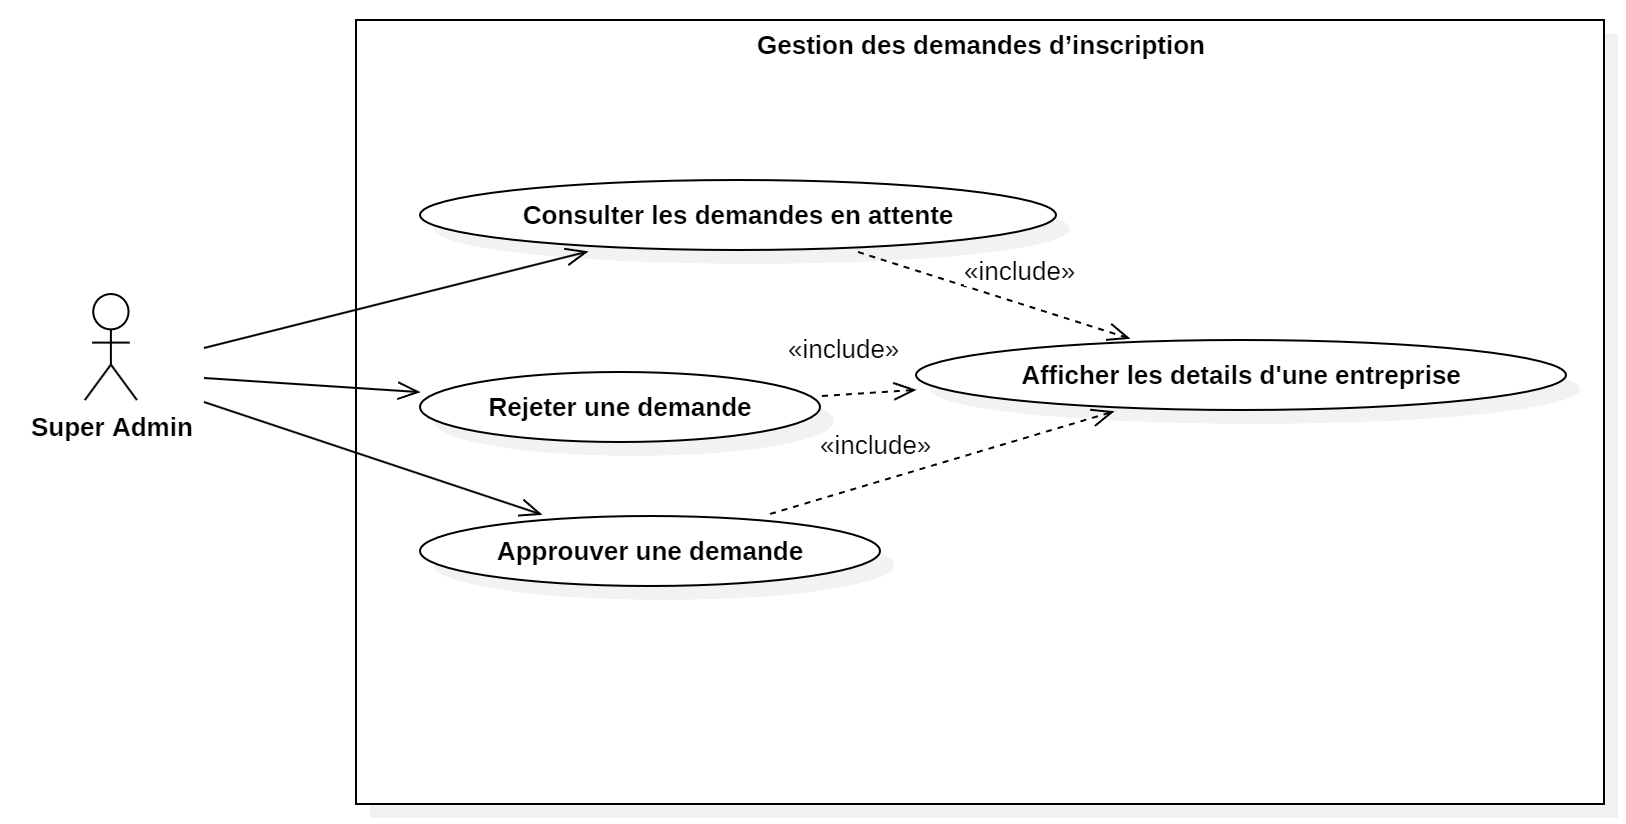
\includegraphics[width=12cm,height=10cm]{images/approveuc.png}
    \caption{Diagramme de cas d'utilisation - Gestion des demandes d'inscription}
\end{figure}
\vspace{\baselineskip}
\vspace{\baselineskip}

\begin{longtable}{|>{\raggedright\arraybackslash}p{4cm}|>{\raggedright\arraybackslash}p{9cm}|}
\caption{Description textuelle du cas d'utilisation - Gestion des demandes d'inscription}
\label{tab:manage_requests_usecase} \\
\hline
\textbf{Cas d'utilisation} & \textbf{Gérer les demandes d'inscription} \\
\hline
\textbf{Acteur} & Super Admin \\
\hline
\textbf{Précondition} & Être authentifié en tant que Super Admin \\
\hline
\textbf{Postcondition} & Statut de l'entreprise modifié (Approuvé/Rejeté) \\
\hline
\textbf{Scénario nominal} & 
1. Le Super Admin accède à la page des demandes en attente \\
& 2. Le système affiche la liste des entreprises en attente \\
& 3. Le Super Admin consulte les détails d'une demande \\
& 4. Le Super Admin décide d'approuver ou rejeter \\
& 5. Le système met à jour le statut de l'entreprise \\
& 6. Le système affiche un message de confirmation \\
\hline
\textbf{Scénario alternatif} & 
- Aucune demande en attente : affichage d'un message informatif \\
& - Erreur de traitement : affichage d'un message d'erreur \\
& - Perte de session : redirection vers l'authentification \\
\hline
\end{longtable}

\subsubsection{Diagramme de cas d'utilisation détaillé de la gestion des profils}
\noindent La figure 4.4 présente le diagramme de cas d'utilisation pour la gestion des profils utilisateur.

\begin{figure}[H]
    \centering
    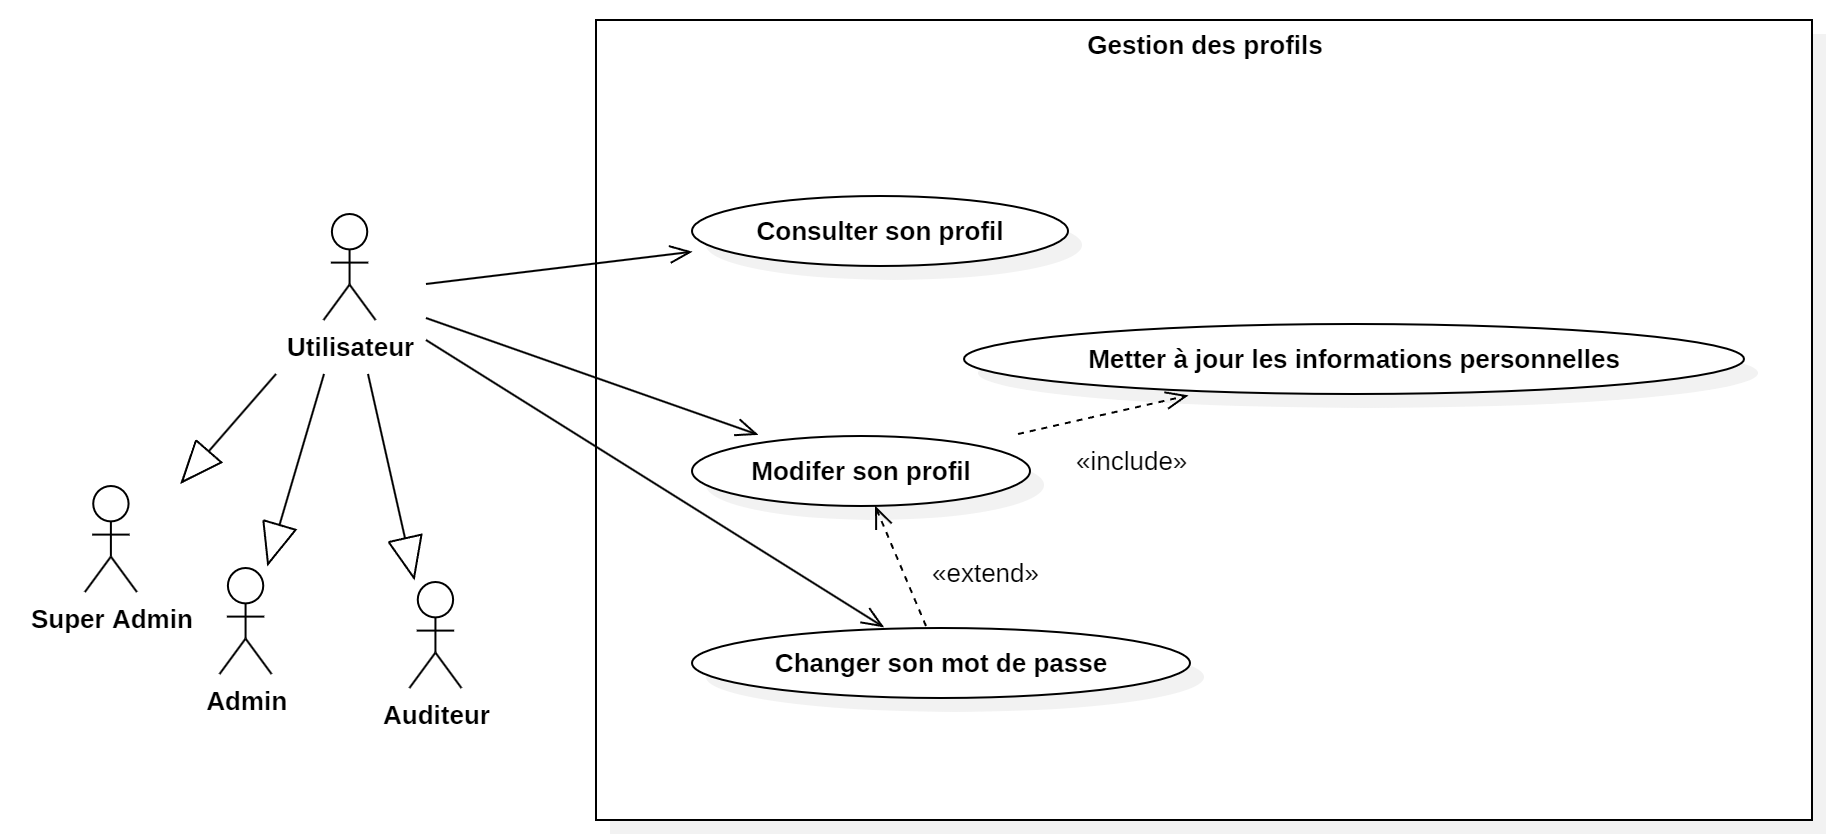
\includegraphics[width=12cm,height=8cm]{images/profileuc.png}
    \caption{Diagramme de cas d'utilisation - Gestion des profils}
\end{figure}
\begin{longtable}{|>{\raggedright\arraybackslash}p{4cm}|>{\raggedright\arraybackslash}p{10cm}|}
\caption{Description textuelle du cas d'utilisation - Gestion des profils}
\label{tab:manage_profile_usecase} \\
\hline
\textbf{Cas d'utilisation} & \textbf{Gérer son profil} \\
\hline
\textbf{Acteur} & Super Admin, Admin, Auditeur \\
\hline
\textbf{Précondition} & Être authentifié dans le système \\
\hline
\textbf{Postcondition} & Informations du profil mises à jour \\
\hline
\textbf{Scénario nominal} & 
1. L'utilisateur accède à la page de profil \\
& 2. Le système affiche les informations actuelles \\
& 3. L'utilisateur modifie les champs souhaités \\
& 4. L'utilisateur sauvegarde les modifications \\
& 5. Le système valide les données \\
& 6. Le système met à jour les informations \\
& 7. Le système affiche un message de confirmation \\
\hline
\textbf{Scénario alternatif} & 
- Modification du mot de passe : vérification de l'ancien mot de passe \\
& - Données invalides : affichage des erreurs de validation \\
& - Échec de sauvegarde : affichage d'un message d'erreur \\
\hline
\end{longtable}

\subsection{Conception}
\noindent Dans cette partie, nous passons à la seconde phase de notre sprint. Notre objectif est de créer les diagrammes de séquence correspondant à cette étape.

\subsubsection{Diagramme de séquence}

\subsubsection{Diagramme de séquence pour le scénario d'authentification}
\begin{figure}[H]
    \centering
    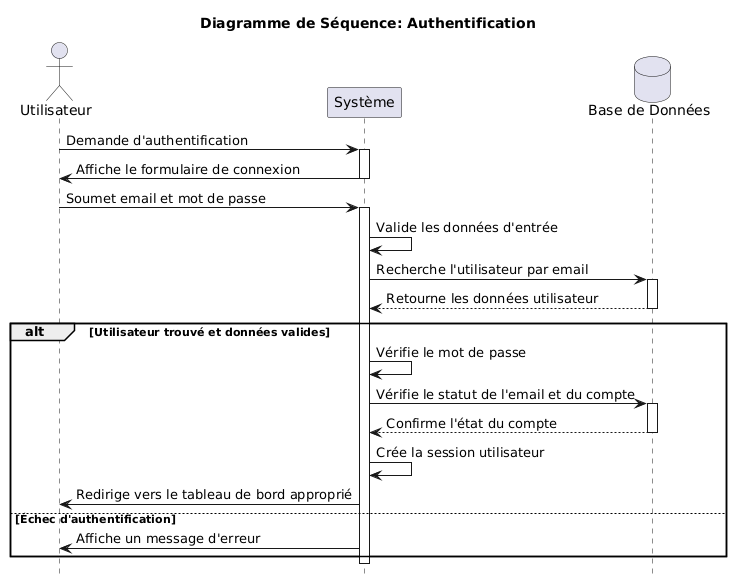
\includegraphics[width=10cm,height=9cm]{images/authentifiaction.png}
    \caption{Diagramme de séquence pour le scénario d'authentification}
\end{figure}

\subsubsection{Diagramme de séquence pour le scénario d'inscription}
\begin{figure}[H]
    \centering
    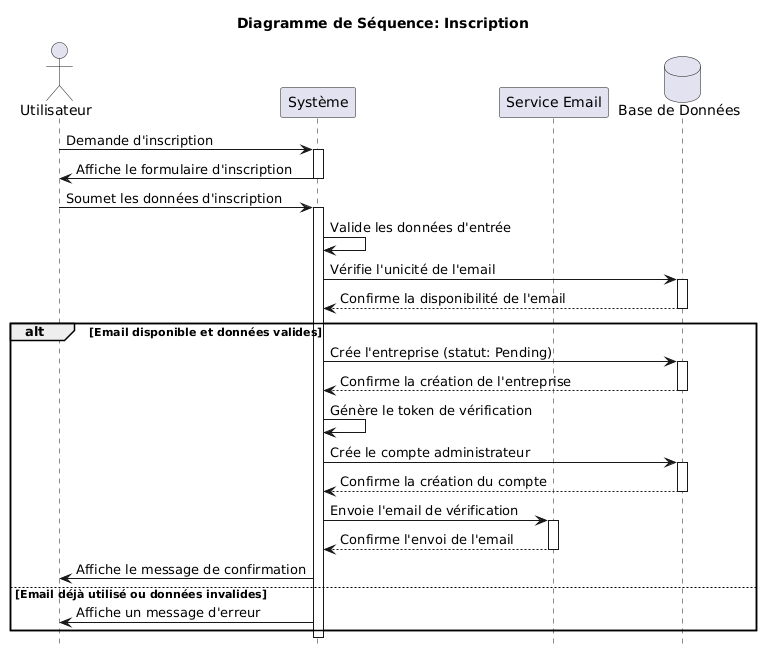
\includegraphics[width=10cm,height=9cm]{images/inscription.png}
    \caption{Diagramme de séquence pour le scénario d'inscription}
\end{figure}

\subsubsection{Diagramme de séquence pour le scénario d'approbation des demandes}
\begin{figure}[H]
    \centering
    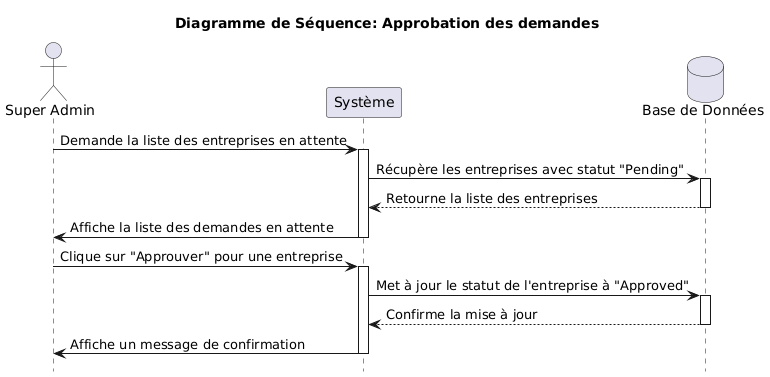
\includegraphics[width=10cm,height=6cm]{images/demandeseq.png}
    \caption{Diagramme de séquence pour le scénario d'approbation des demandes}
\end{figure}

\subsubsection{Diagramme de séquence pour le scénario de modification du profil}
\begin{figure}[H]
    \centering
    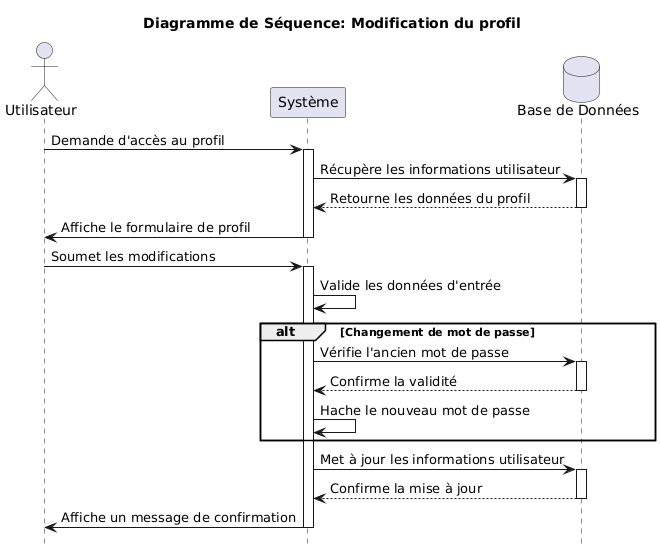
\includegraphics[width=10cm,height=9cm]{images/profilseq.png}
    \caption{Diagramme de séquence pour le scénario de modification du profil}
\end{figure}

\subsection{Réalisation}
\noindent Dans cette section, nous vous présenterons les résultats de ce sprint sous forme d'une série de captures d'écran illustrant différentes interfaces que nous avons développées.

\subsubsection{Interface d'authentification}
\noindent La figure 4.9 présente l'interface d'authentification permettant aux utilisateurs de se connecter au système.

\begin{figure}[H]
    \centering
    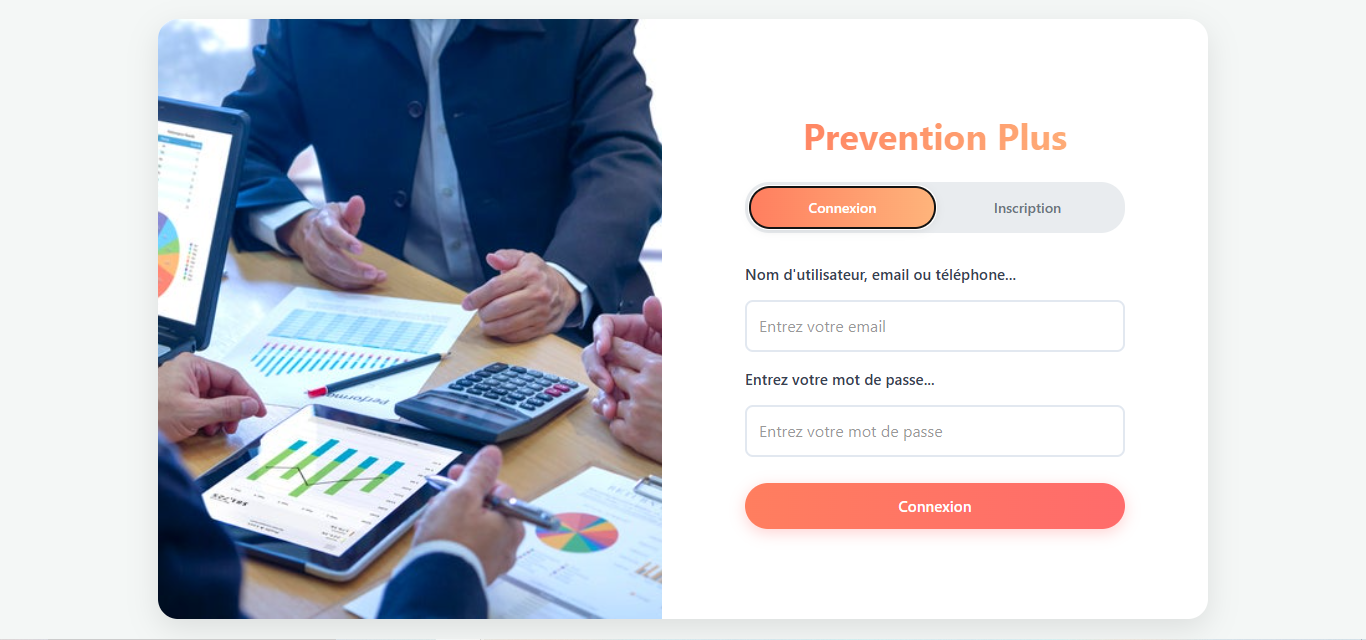
\includegraphics[width=17cm,height=11cm]{images/authpic.PNG}
    \caption{Interface d'authentification}
\end{figure}

\subsubsection{Interface d'inscription}
\noindent La figure 4.10 présente l'interface d'inscription permettant aux entreprises de créer leur compte.

\begin{figure}[H]
    \centering
    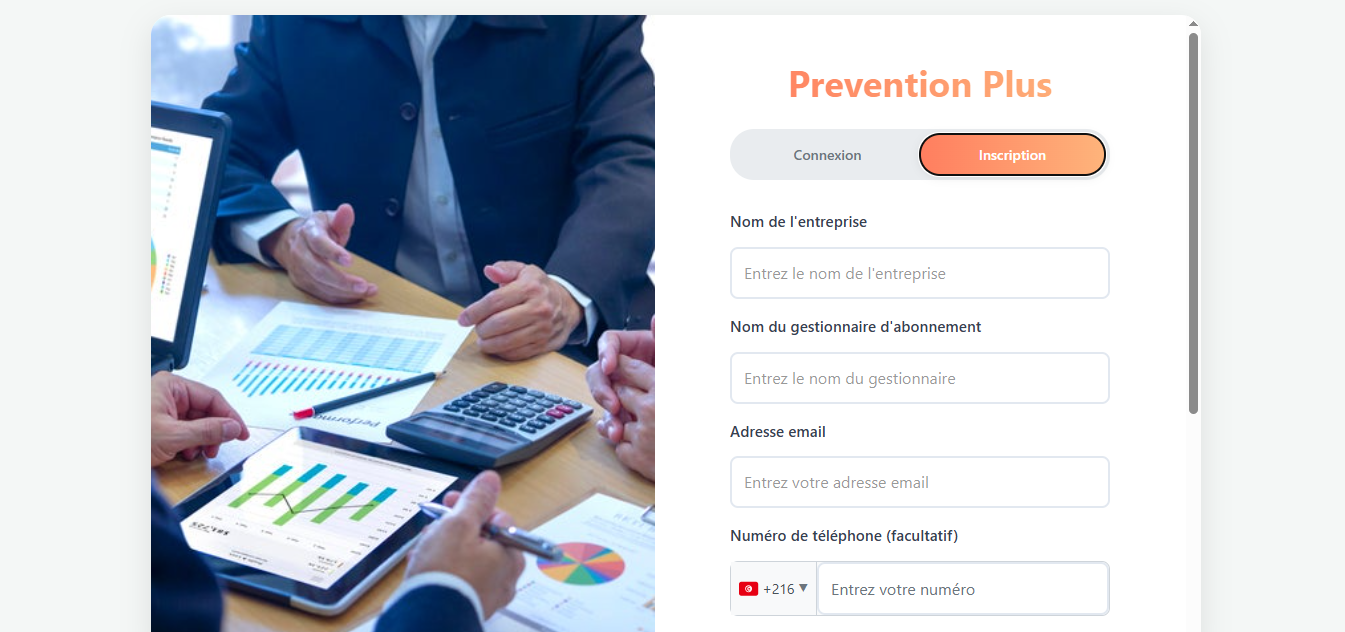
\includegraphics[width=15cm,height=9cm]{images/inscpic.PNG}
    \caption{Interface d'inscription}
\end{figure}


\subsubsection{Interface de gestion des demandes d'inscription}
\noindent La figure 4.11 présente l'interface permettant au Super Admin de gérer les demandes d'inscription en attente.

\begin{figure}[H]
    \centering
    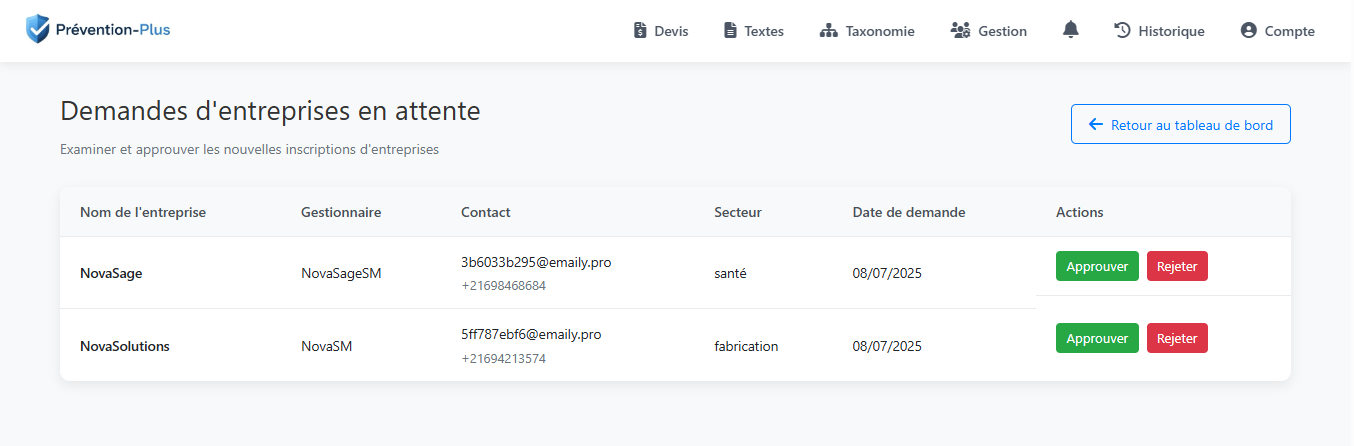
\includegraphics[width=15cm,height=8cm]{images/approvepic.PNG}
    \caption{Interface de gestion des demandes d'inscription}
\end{figure}

\subsubsection{Interface de gestion des profils}
\noindent La figure 4.12 présente l'interface de gestion des profils utilisateur.

\begin{figure}[H]
    \centering
    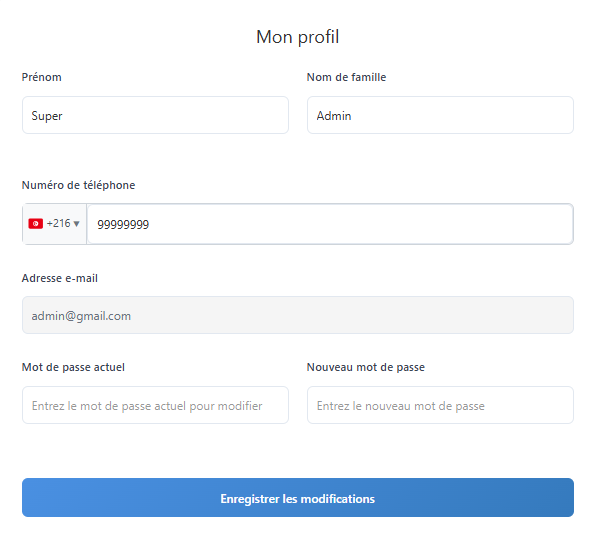
\includegraphics[width=14cm,height=9cm]{images/profilepic.PNG}
    \caption{Interface de gestion des profils}
\end{figure}

\section{Sprint 2 : Gestion des utilisateurs, entreprises, paramètres d'entreprise et taxonomie}

\subsection{Spécifications fonctionnelles}
\noindent Ce sprint représente la deuxième phase de notre premier release, établissant les mécanismes de gestion des utilisateurs, entreprises, paramètres d'entreprise et taxonomie.

\subsubsection{Backlog du Sprint 2}
\noindent Le sprint backlog est constitué à partir du backlog produit présenté au chapitre 2. Pour ce deuxième sprint, nous avons sélectionné les user stories présentées dans le tableau 4.7.

\begin{longtable}{|>{\raggedright\arraybackslash}p{4cm}|>{\raggedright\arraybackslash}p{7cm}|>{\raggedright\arraybackslash}p{2cm}|}
\caption{Backlog du sprint 2}
\label{tab:sprint2_backlog}\\
\hline
Histoire utilisateur & Description & Priorité \\
\hline
\endfirsthead
\multicolumn{3}{c}{\tablename\ \thetable\ -- suite} \\
\hline
Histoire utilisateur & Description & Priorité \\
\hline
\endhead
Créer des utilisateurs & En tant qu'Admin, je veux créer des utilisateurs dans mon entreprise pour organiser mon équipe & Élevée \\
\hline
Consulter les utilisateurs & En tant qu'Admin, je veux consulter les utilisateurs de mon entreprise & Élevée \\
\hline
Modifier les utilisateurs & En tant qu'Admin, je veux modifier les utilisateurs de mon entreprise & Moyenne \\
\hline
Supprimer les utilisateurs & En tant qu'Admin, je veux supprimer les utilisateurs de mon entreprise & Moyenne \\
\hline
Consulter tous les utilisateurs & En tant que Super Admin, je veux consulter tous les utilisateurs du système & Moyenne \\
\hline
Supprimer les utilisateurs (Super Admin) & En tant que Super Admin, je veux supprimer les utilisateurs pour administrer le système & Moyenne \\
\hline
Consulter les entreprises & En tant que Super Admin, je veux consulter toutes les entreprises pour administrer la plateforme & Moyenne \\
\hline
Supprimer les entreprises & En tant que Super Admin, je veux supprimer les entreprises pour administrer la plateforme & Moyenne \\
\hline
Consulter les paramètres d'entreprise & En tant que Admin, je veux consulter les paramètres de mon entreprise pour visualiser la configuration & Moyenne \\
\hline
Modifier les paramètres d'entreprise & En tant que Admin, je veux modifier les paramètres de mon entreprise pour personnaliser la configuration & Moyenne \\
\hline
Créer des éléments de taxonomie & En tant que Super Admin, je veux créer des éléments de taxonomie pour organiser la classification du système & Élevée \\
\hline
Consulter la taxonomie & En tant que Super Admin, je veux consulter la taxonomie pour superviser la classification & Élevée \\
\hline
Modifier des éléments de taxonomie & En tant que Super Admin, je veux modifier des éléments de taxonomie pour maintenir l'organisation du système & Moyenne \\
\hline
Supprimer des éléments de taxonomie & En tant que Super Admin, je veux supprimer des éléments de taxonomie pour maintenir l'organisation du système & Moyenne \\
\hline
Générer des suggestions de taxonomie & En tant que Super Admin, je veux générer des suggestions de taxonomie par IA pour optimiser la classification & Faible \\
\hline
\end{longtable}

\subsubsection{Diagramme de cas d'utilisation détaillé de la gestion des utilisateurs}
\noindent La figure 4.13 présente le diagramme de cas d'utilisation détaillé pour la gestion des utilisateurs par l'Admin et le Super Admin.

\begin{figure}[H]
    \centering
    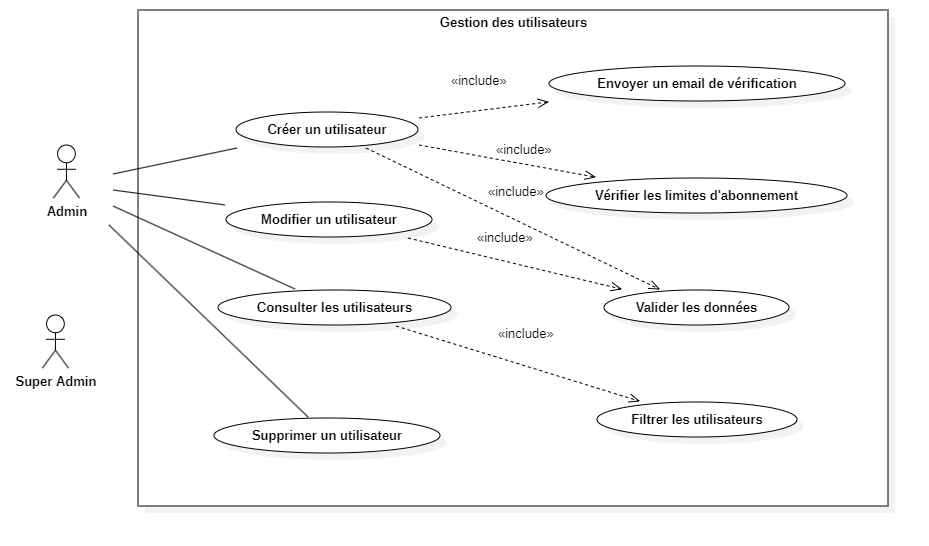
\includegraphics[width=13cm,height=8cm]{images/gestionuseruc.png}
    \caption{Diagramme de cas d'utilisation - Gestion des utilisateurs}
\end{figure}

\begin{longtable}{|>{\raggedright\arraybackslash}p{4cm}|>{\raggedright\arraybackslash}p{9cm}|}
\caption{Description textuelle du cas d'utilisation - Gestion des utilisateurs}
\label{tab:manage_users_usecase} \\
\hline
\textbf{Cas d'utilisation} & \textbf{Gérer les utilisateurs} \\
\hline
\textbf{Acteur} & Admin, Super Admin \\
\hline
\textbf{Précondition} & Être authentifié dans le système \\
\hline
\textbf{Postcondition} & Utilisateurs créés, modifiés ou supprimés selon l'action \\
\hline
\textbf{Scénario nominal} & 
1. L'acteur accède à la page de gestion des utilisateurs \\
& 2. Le système affiche la liste des utilisateurs appropriée \\
& 3. L'acteur sélectionne une action (créer, modifier, supprimer) \\
& 4. Le système affiche le formulaire correspondant \\
& 5. L'acteur saisit ou modifie les informations \\
& 6. Le système valide les données \\
& 7. Le système met à jour la base de données \\
& 8. Le système affiche un message de confirmation \\
\hline
\textbf{Scénario alternatif} & 
- Création : vérification de l'unicité de l'email \\
& - Modification : protection des rôles Admin \\
& - Suppression : vérification des contraintes de suppression \\
& - Limite d'abonnement atteinte : refus de création \\
\hline
\end{longtable}

\subsubsection{Diagramme de cas d'utilisation détaillé de la gestion des entreprises}
\noindent La figure 4.14 présente le diagramme de cas d'utilisation détaillé pour la gestion des entreprises par le Super Admin.

\begin{figure}[H]
    \centering
    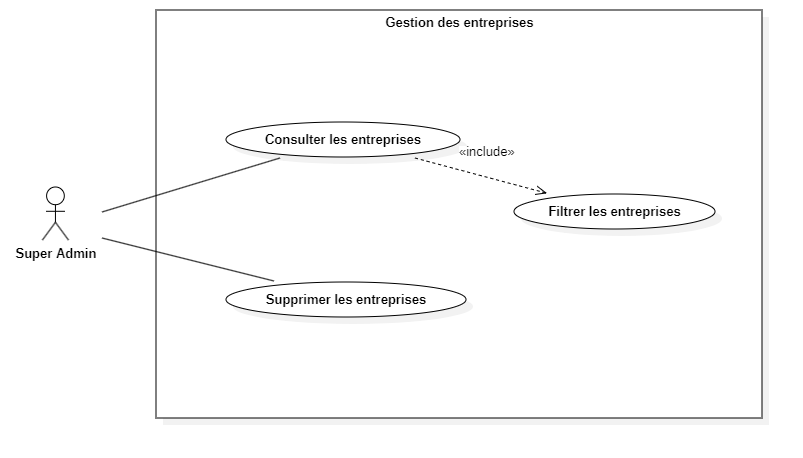
\includegraphics[width=12cm,height=8cm]{images/gestioncompanyuc.png}
    \caption{Diagramme de cas d'utilisation - Gestion des entreprises}
\end{figure}

\begin{longtable}{|>{\raggedright\arraybackslash}p{4cm}|>{\raggedright\arraybackslash}p{9cm}|}
\caption{Description textuelle du cas d'utilisation - Gestion des entreprises}
\label{tab:manage_companies_usecase} \\
\hline
\textbf{Cas d'utilisation} & \textbf{Gérer les entreprises} \\
\hline
\textbf{Acteur} & Super Admin \\
\hline
\textbf{Précondition} & Être authentifié en tant que Super Admin \\
\hline
\textbf{Postcondition} & Entreprises consultées ou supprimées selon l'action \\
\hline
\textbf{Scénario nominal} & 
1. Le Super Admin accède à la page de gestion des entreprises \\
& 2. Le système affiche la liste détaillée des entreprises \\
& 3. Le Super Admin peut filtrer et rechercher les entreprises \\
& 4. Le Super Admin sélectionne une action (consulter, supprimer) \\
& 5. Le système exécute l'action demandée \\
& 6. Le système affiche un message de confirmation \\
\hline
\textbf{Scénario alternatif} & 
- Suppression : vérification des données associées \\
& - Aucune entreprise trouvée : affichage d'un message informatif \\
& - Erreur de traitement : affichage d'un message d'erreur \\
& - Suppression avec cascade : suppression des utilisateurs et données associées \\
\hline
\end{longtable}

\subsubsection{Diagramme de cas d'utilisation détaillé de la gestion des paramètres d'entreprise}
\noindent La figure 4.15 présente le diagramme de cas d'utilisation détaillé pour la gestion des paramètres d'entreprise par l'Admin.

\begin{figure}[H]
    \centering
    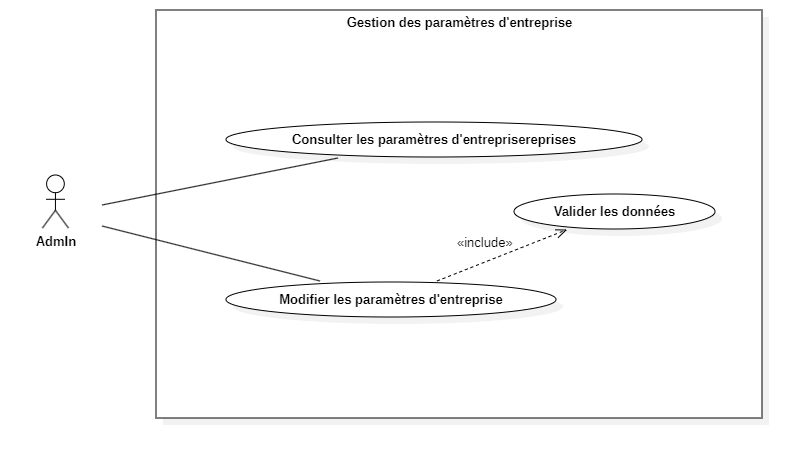
\includegraphics[width=12cm,height=8cm]{images/gestionparamcompanyuc.png}
    \caption{Diagramme de cas d'utilisation - Gestion des paramètres d'entreprise}
\end{figure}

\begin{longtable}{|>{\raggedright\arraybackslash}p{4cm}|>{\raggedright\arraybackslash}p{9cm}|}
\caption{Description textuelle du cas d'utilisation - Gestion des paramètres d'entreprise}
\label{tab:manage_company_settings_usecase} \\
\hline
\textbf{Cas d'utilisation} & \textbf{Gérer les paramètres d'entreprise} \\
\hline
\textbf{Acteur} & Admin \\
\hline
\textbf{Précondition} & Être authentifié en tant qu'Admin \\
\hline
\textbf{Postcondition} & Paramètres d'entreprise consultés ou modifiés \\
\hline
\textbf{Scénario nominal} & 
1. L'Admin accède à la page des paramètres d'entreprise \\
& 2. Le système affiche les informations actuelles de l'entreprise \\
& 3. L'Admin modifie les champs souhaités \\
& 4. L'Admin soumet les modifications \\
& 5. Le système valide les données \\
& 6. Le système met à jour les informations \\
& 7. Le système affiche un message de confirmation \\
\hline
\textbf{Scénario alternatif} & 
- Données invalides : affichage des erreurs de validation \\
& - Nom d'entreprise vide : message d'erreur \\
& - Secteur non sélectionné : message d'erreur \\
& - Échec de sauvegarde : affichage d'un message d'erreur \\
\hline
\end{longtable}

\subsubsection{Diagramme de cas d'utilisation détaillé de la gestion de la taxonomie}
\noindent La figure 4.16 présente le diagramme de cas d'utilisation détaillé pour la gestion de la taxonomie par le Super Admin.

\begin{figure}[H]
    \centering
    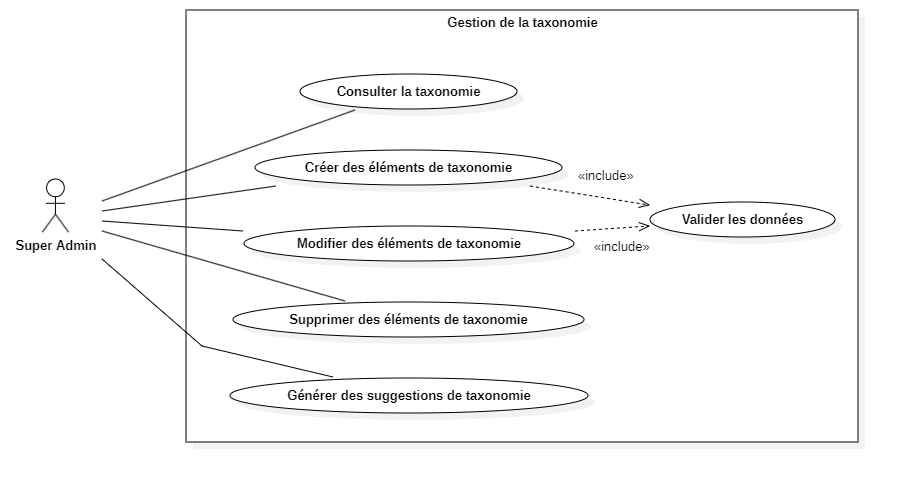
\includegraphics[width=12cm,height=7cm]{images/taxonomyuc.png}
    \caption{Diagramme de cas d'utilisation - Gestion de la taxonomie}
\end{figure}

\begin{longtable}{|>{\raggedright\arraybackslash}p{4cm}|>{\raggedright\arraybackslash}p{9cm}|}
\caption{Description textuelle du cas d'utilisation - Gestion de la taxonomie}
\label{tab:manage_taxonomy_usecase} \\
\hline
\textbf{Cas d'utilisation} & \textbf{Gérer la taxonomie} \\
\hline
\textbf{Acteur} & Super Admin \\
\hline
\textbf{Précondition} & Être authentifié en tant que Super Admin \\
\hline
\textbf{Postcondition} & Éléments de taxonomie créés, modifiés ou supprimés selon l'action \\
\hline
\textbf{Scénario nominal} & 
1. Le Super Admin accède à la page de gestion de la taxonomie \\
& 2. Le système affiche la structure hiérarchique de la taxonomie \\
& 3. Le Super Admin sélectionne une action (créer, modifier, supprimer) \\
& 4. Le système affiche le formulaire correspondant \\
& 5. Le Super Admin saisit ou modifie les informations \\
& 6. Le système valide les données et vérifie les contraintes \\
& 7. Le système met à jour la base de données \\
& 8. Le système affiche un message de confirmation \\
\hline
\textbf{Scénario alternatif} & 
- Création : vérification de l'unicité des noms dans le même niveau \\
& - Suppression : vérification des dépendances avec les textes \\
& - Suppression cascade : suppression des éléments enfants \\
& - Génération de suggestion IA : création automatique de taxonomie \\
\hline
\end{longtable}

\subsection{Conception}
\noindent Dans cette partie, nous passons à la seconde phase de notre sprint. Notre objectif est de créer les diagrammes de séquence correspondant à cette étape.


\subsubsection{Diagramme de séquence pour le scénario de création d'utilisateur}
\begin{figure}[H]
    \centering
    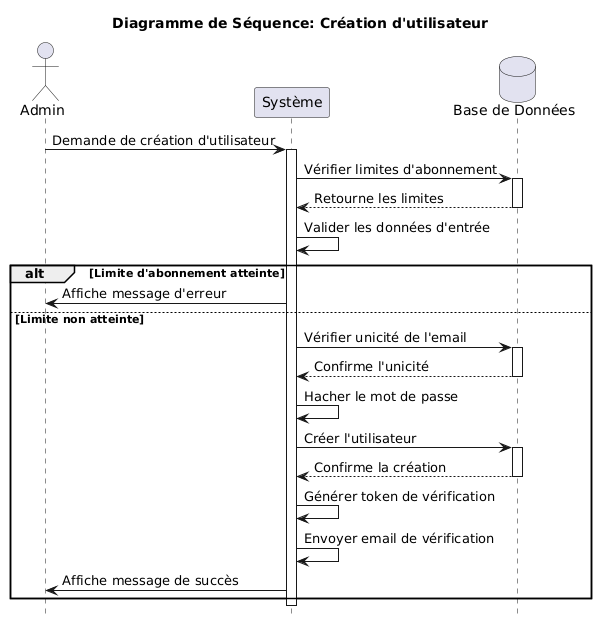
\includegraphics[width=10cm,height=9cm]{images/createusersq.png}
    \caption{Diagramme de séquence pour le scénario de création d'utilisateur}
\end{figure}

\subsubsection{Diagramme de séquence pour le scénario de consultation des utilisateurs}
\begin{figure}[H]
    \centering
    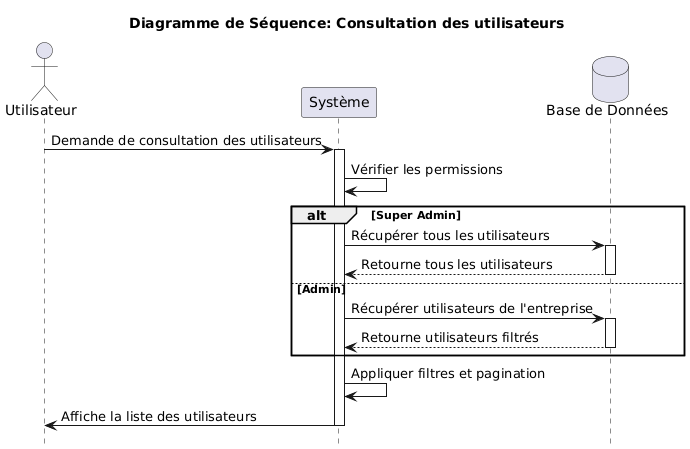
\includegraphics[width=10cm,height=9cm]{images/consultusersq.png}
    \caption{Diagramme de séquence pour le scénario de consultation des utilisateurs}
\end{figure}

\subsubsection{Diagramme de séquence pour le scénario de modification d'utilisateur}
\begin{figure}[H]
    \centering
    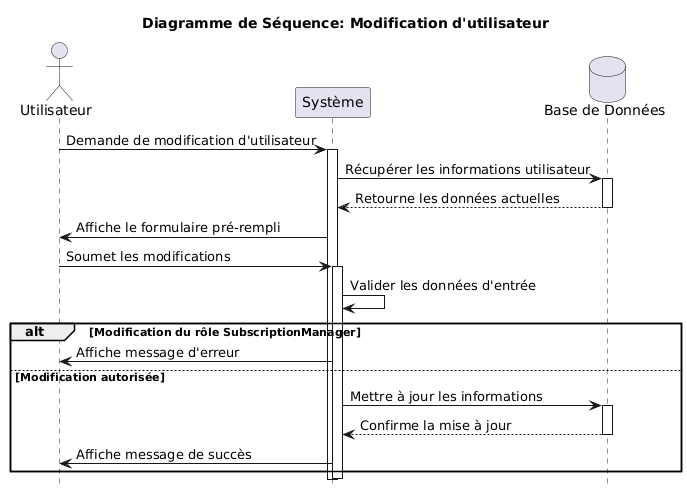
\includegraphics[width=10cm,height=9cm]{images/modifyusersq.png}
    \caption{Diagramme de séquence pour le scénario de modification d'utilisateur}
\end{figure}

\subsubsection{Diagramme de séquence pour le scénario de suppression d'utilisateur}
\begin{figure}[H]
    \centering
    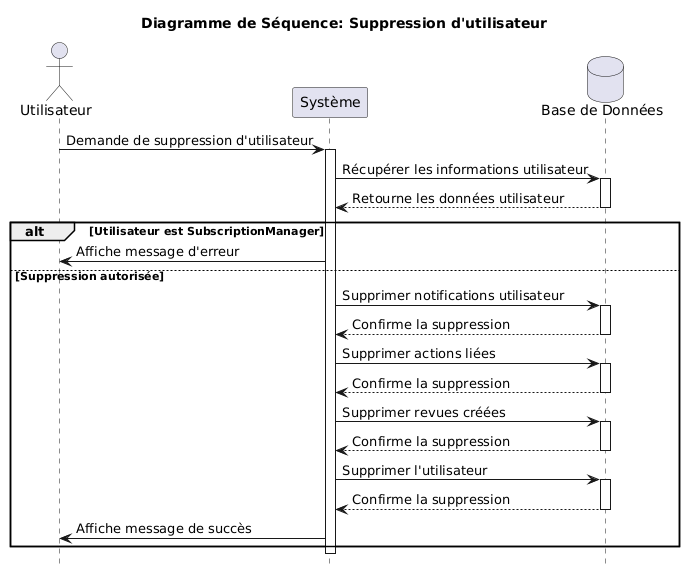
\includegraphics[width=10cm,height=9cm]{images/suppressionutilisateursq.png}
    \caption{Diagramme de séquence pour le scénario de suppression d'utilisateur}
\end{figure}

\subsubsection{Diagramme de séquence pour le scénario de consultation des entreprises}
\begin{figure}[H]
    \centering
    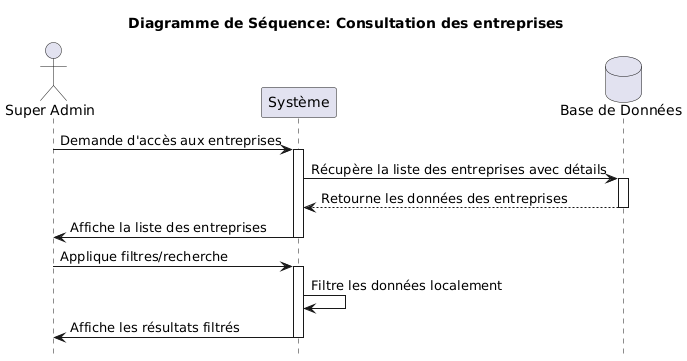
\includegraphics[width=10cm,height=8cm]{images/consultcompanysq.png}
    \caption{Diagramme de séquence pour le scénario de consultation des entreprises}
\end{figure}

\subsubsection{Diagramme de séquence pour le scénario de suppression d'entreprise}
\begin{figure}[H]
    \centering
    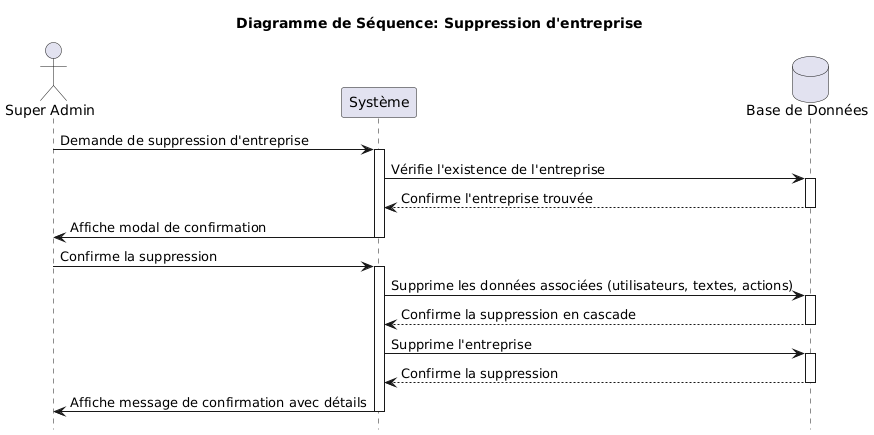
\includegraphics[width=11cm,height=9cm]{images/deletecompanysq.png}
    \caption{Diagramme de séquence pour le scénario de suppression d'entreprise}
\end{figure}

\subsubsection{Diagramme de séquence pour le scénario de consultation des paramètres d'entreprise}
\begin{figure}[H]
    \centering
    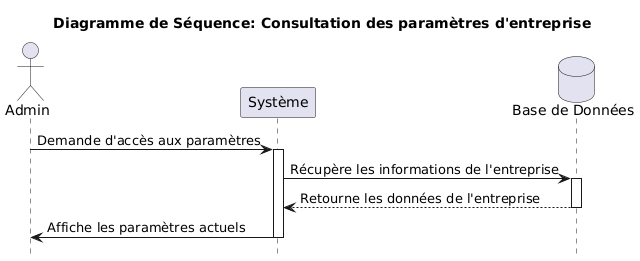
\includegraphics[width=9cm,height=5cm]{images/consultparamcompanysq.png}
    \caption{Diagramme de séquence pour le scénario de consultation des paramètres d'entreprise}
\end{figure}

\subsubsection{Diagramme de séquence pour le scénario de modification des paramètres d'entreprise}
\begin{figure}[H]
    \centering
    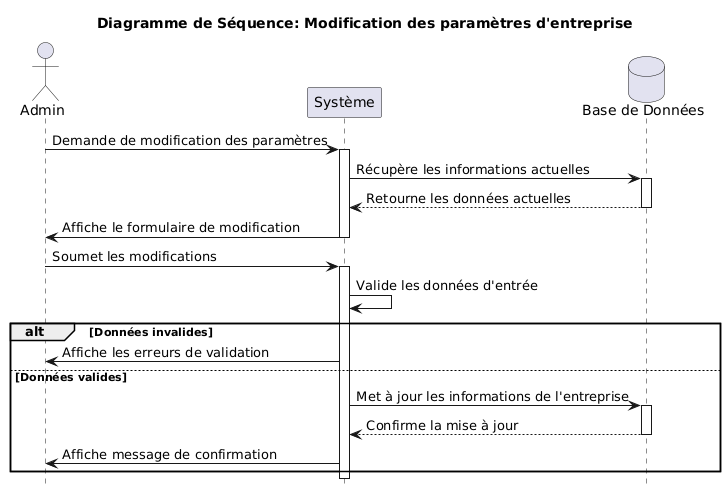
\includegraphics[width=10cm,height=9cm]{images/modifyparamcompanysq.png}
    \caption{Diagramme de séquence pour le scénario de modification des paramètres d'entreprise}
\end{figure}

\subsubsection{Diagramme de séquence pour le scénario de création d'élément de taxonomie}
\begin{figure}[H]
    \centering
    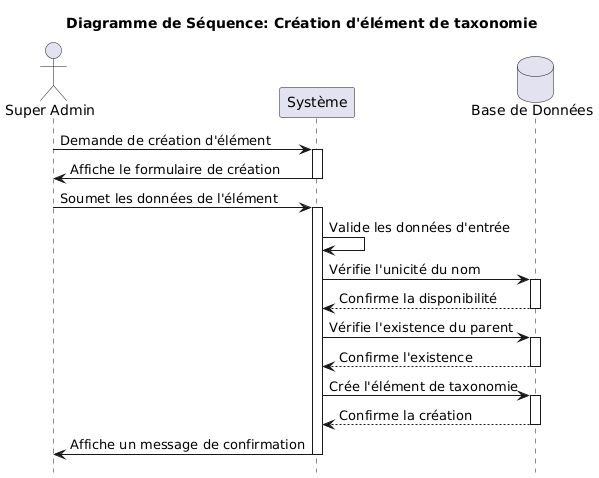
\includegraphics[width=10cm,height=9cm]{images/createtaxonomysq.png}
    \caption{Diagramme de séquence pour le scénario de création d'élément de taxonomie}
\end{figure}

\subsubsection{Diagramme de séquence pour le scénario de consultation de la taxonomie}
\begin{figure}[H]
    \centering
    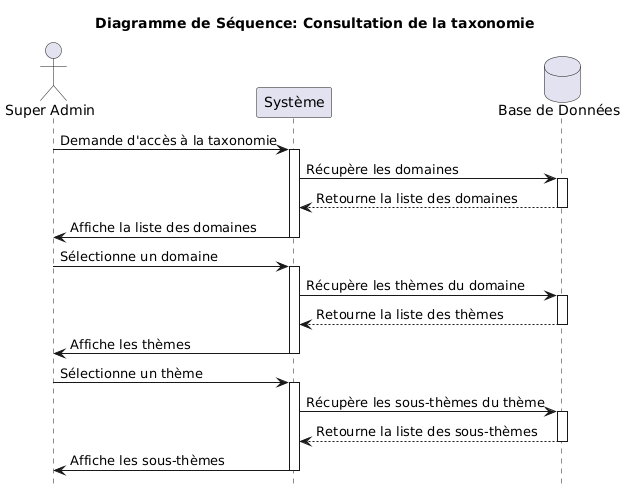
\includegraphics[width=10cm,height=9cm]{images/consulttaxonomysq.png}
    \caption{Diagramme de séquence pour le scénario de consultation de la taxonomie}
\end{figure}

\subsubsection{Diagramme de séquence pour le scénario de modification d'élément de taxonomie}
\begin{figure}[H]
    \centering
    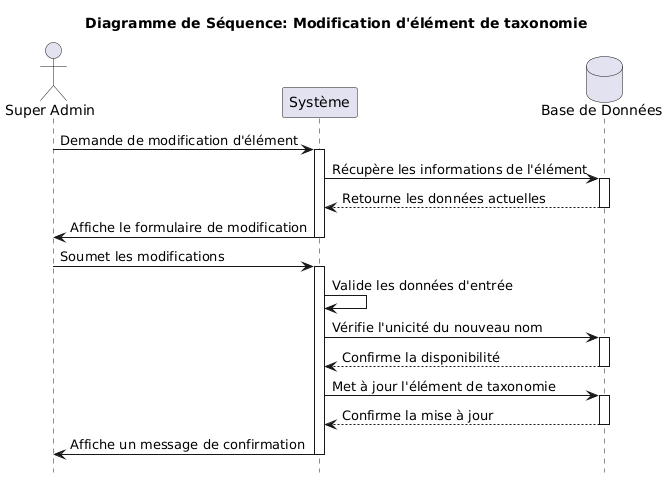
\includegraphics[width=9cm,height=8cm]{images/modifytaxonomysq.png}
    \caption{Diagramme de séquence pour le scénario de modification d'élément de taxonomie}
\end{figure}

\subsubsection{Diagramme de séquence pour le scénario de suppression d'élément de taxonomie}
\begin{figure}[H]
    \centering
    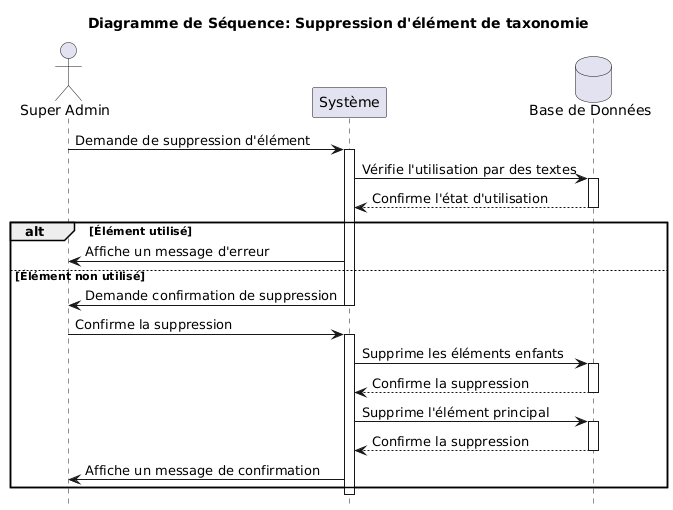
\includegraphics[width=10cm,height=9cm]{images/deletetaxonomysq.png}
    \caption{Diagramme de séquence pour le scénario de suppression d'élément de taxonomie}
\end{figure}

\subsubsection{Diagramme de séquence pour le scénario de génération de suggestion de taxonomie}
\begin{figure}[H]
    \centering
    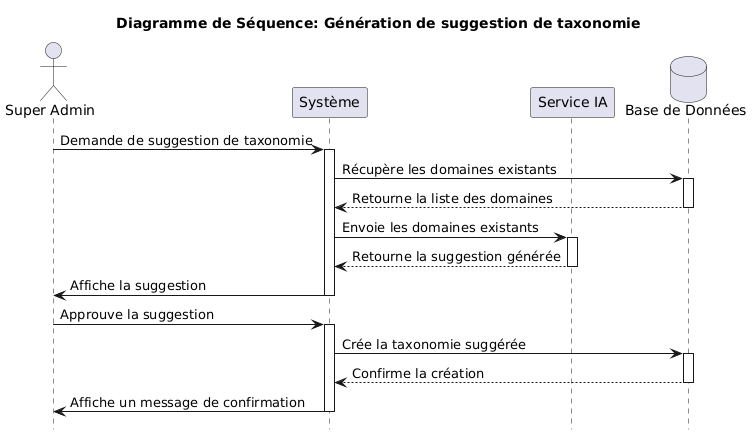
\includegraphics[width=10cm,height=9cm]{images/taxonomyaisq.png}
    \caption{Diagramme de séquence pour le scénario de génération de suggestion de taxonomie}
\end{figure}

\subsection{Réalisation}
\noindent Dans cette section, nous vous présenterons les résultats de ce sprint sous forme d'une série de captures d'écran illustrant différentes interfaces que nous avons développées.

\subsubsection{Interface de gestion des utilisateurs (Admin)}
\noindent La figure 4.24 présente l'interface de gestion des utilisateurs pour l'Admin permettant de créer, modifier et supprimer les utilisateurs de son entreprise.

\begin{figure}[H]
    \centering
    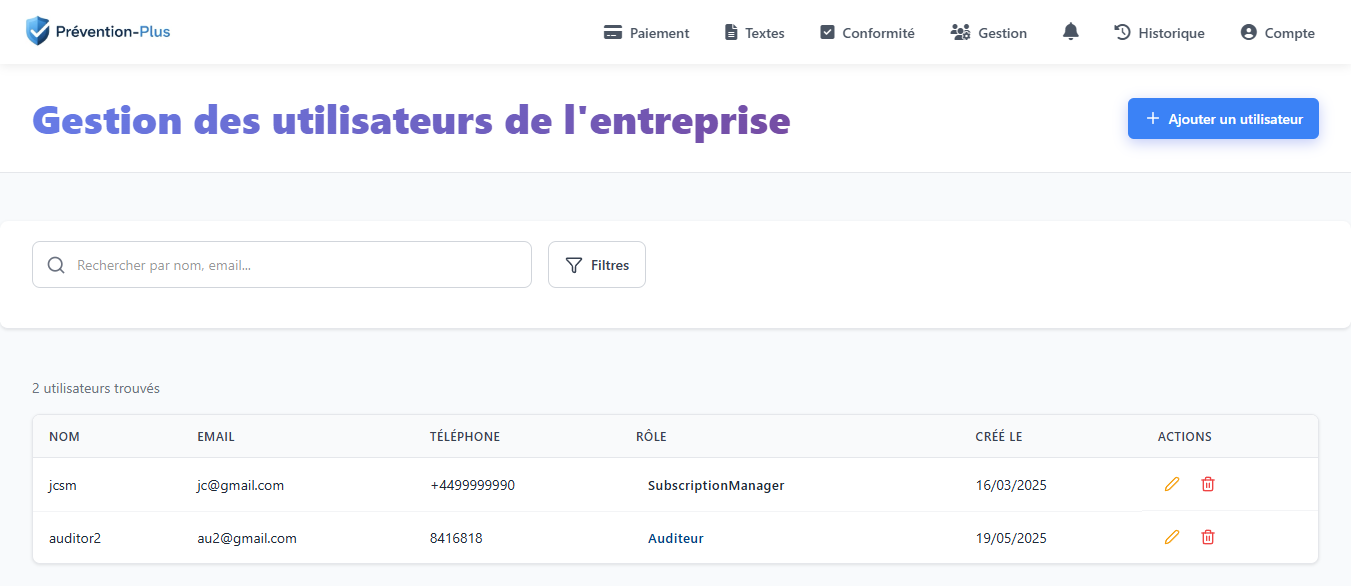
\includegraphics[width=14cm,height=9cm]{images/adminmanageusers.PNG}
    \caption{Interface de gestion des utilisateurs - Admin}
\end{figure}

\subsubsection{Interface de création d'utilisateur}
\noindent La figure 4.25 présente l'interface de création d'un nouvel utilisateur avec tous les champs nécessaires.

\begin{figure}[H]
    \centering
    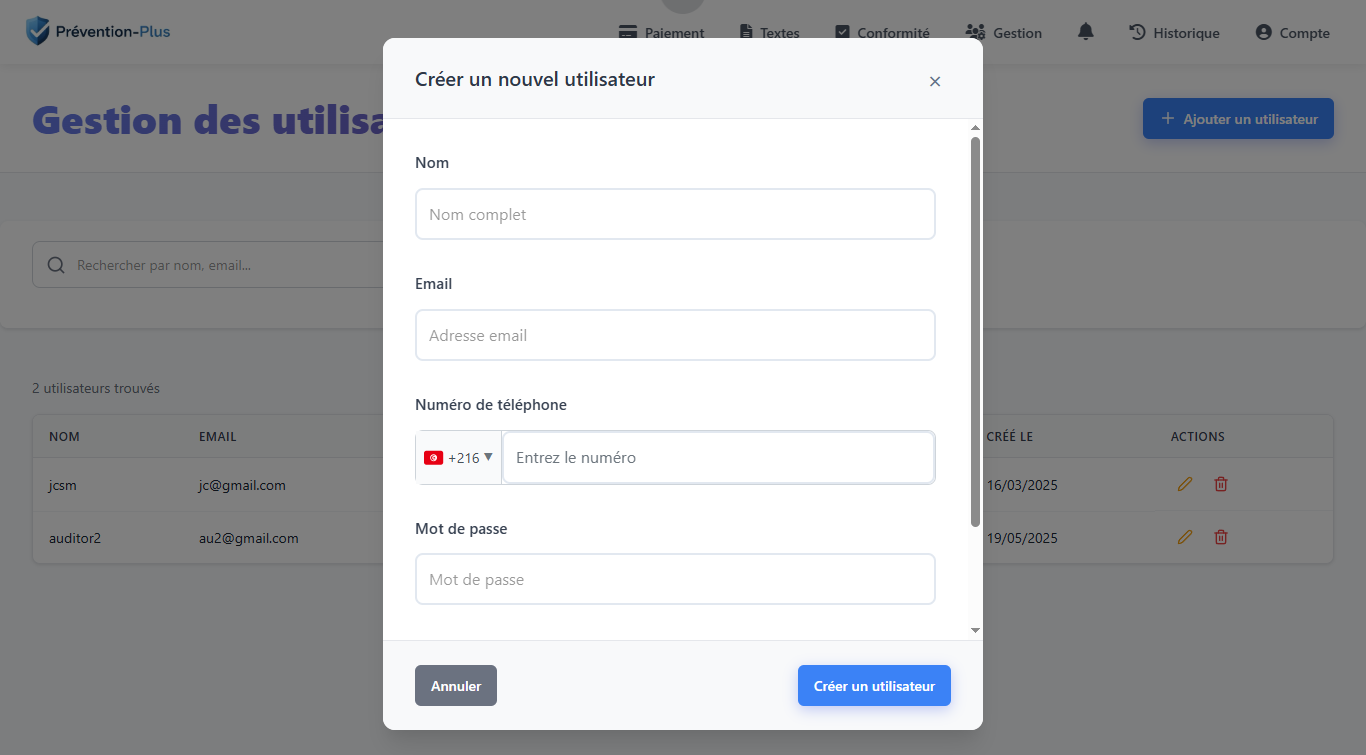
\includegraphics[width=14cm,height=9cm]{images/createusermodal.PNG}
    \caption{Interface de création d'utilisateur}
\end{figure}

\subsubsection{Interface de modification d'utilisateur}
\noindent La figure 4.26 présente l'interface de modification d'un utilisateur existant.

\begin{figure}[H]
    \centering
    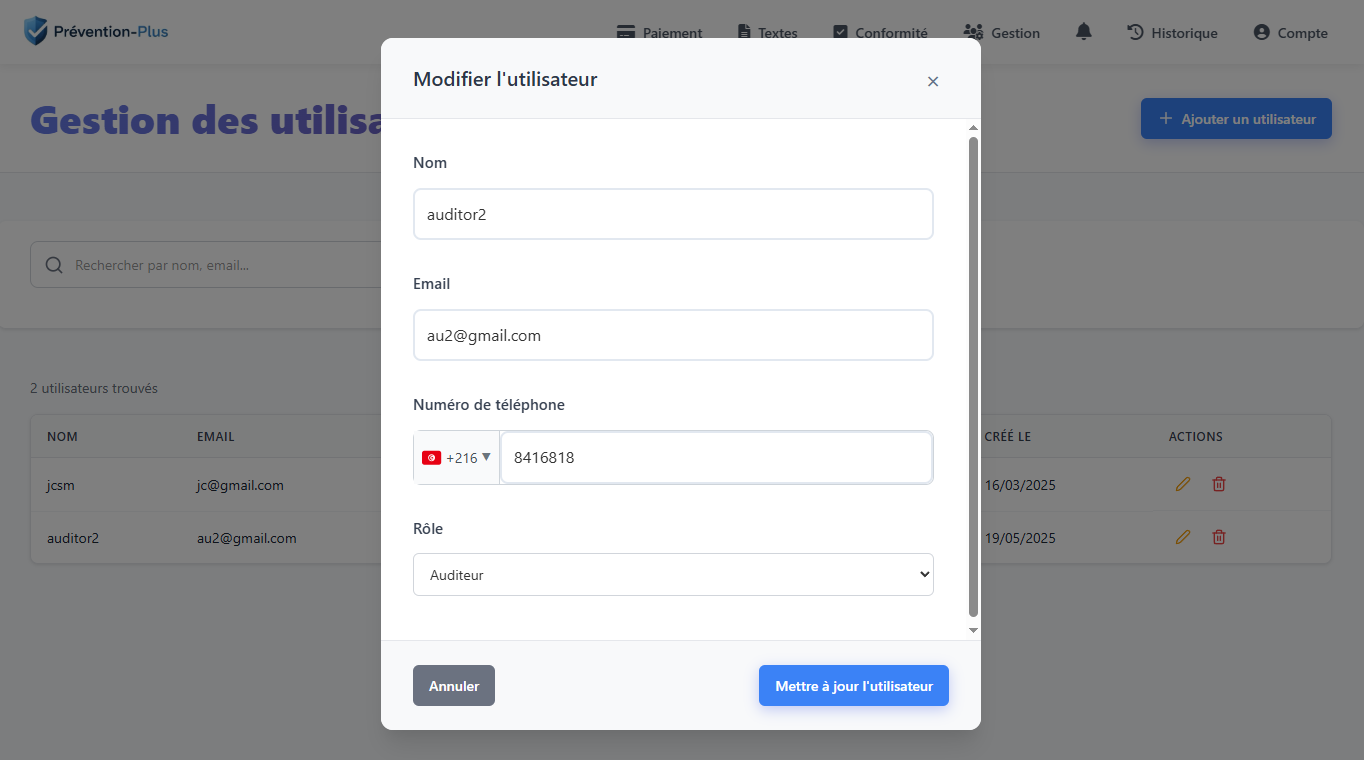
\includegraphics[width=14cm,height=9cm]{images/editusermodal.PNG}
    \caption{Interface de modification d'utilisateur}
\end{figure}

\subsubsection{Interface de gestion des utilisateurs (Super Admin)}
\noindent La figure 4.27 présente l'interface de gestion des utilisateurs pour le Super Admin permettant de consulter et supprimer tous les utilisateurs du système.

\begin{figure}[H]
    \centering
    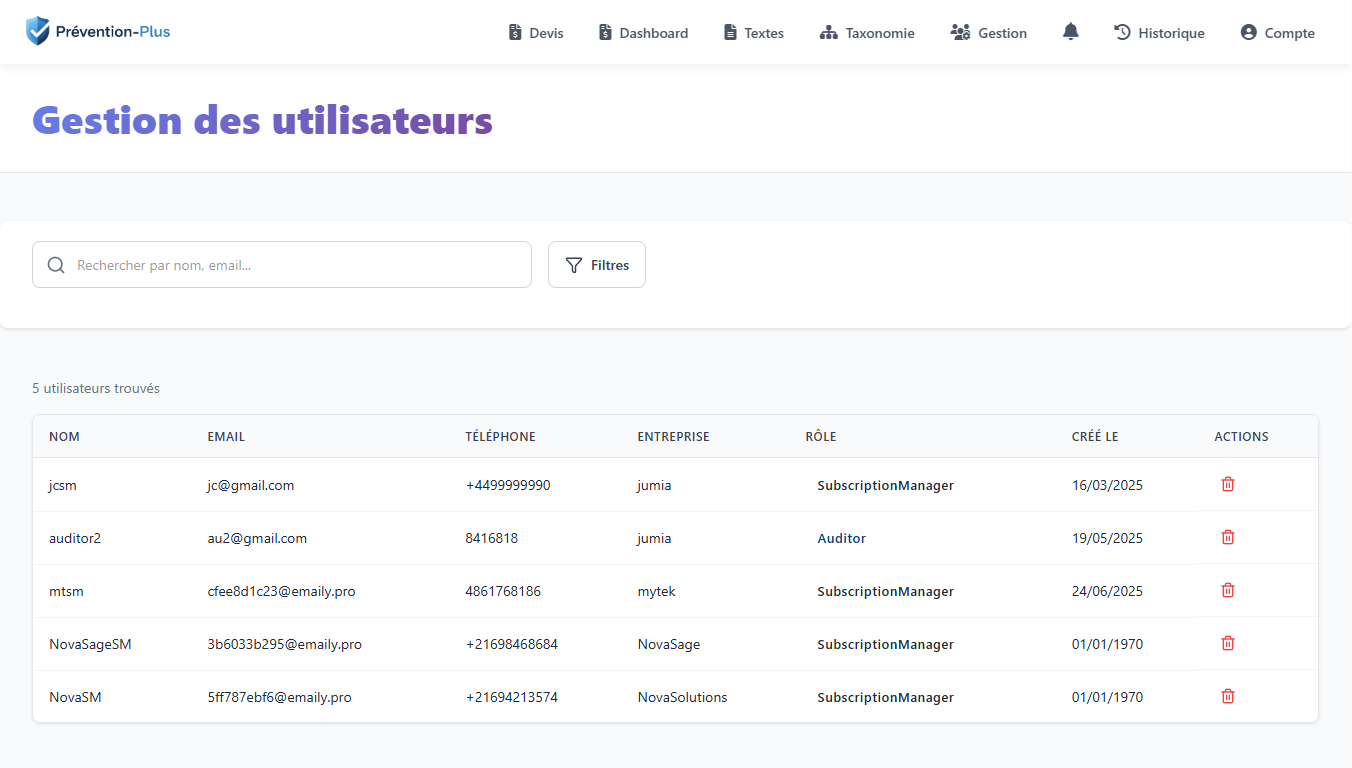
\includegraphics[width=14cm,height=9cm]{images/superadminmanageusers.PNG}
    \caption{Interface de gestion des utilisateurs - Super Admin}
\end{figure}

\subsubsection{Interface de gestion des entreprises}
\noindent La figure 4.28 présente l'interface de gestion des entreprises pour le Super Admin permettant de consulter et supprimer les entreprises.

\begin{figure}[H]
    \centering
    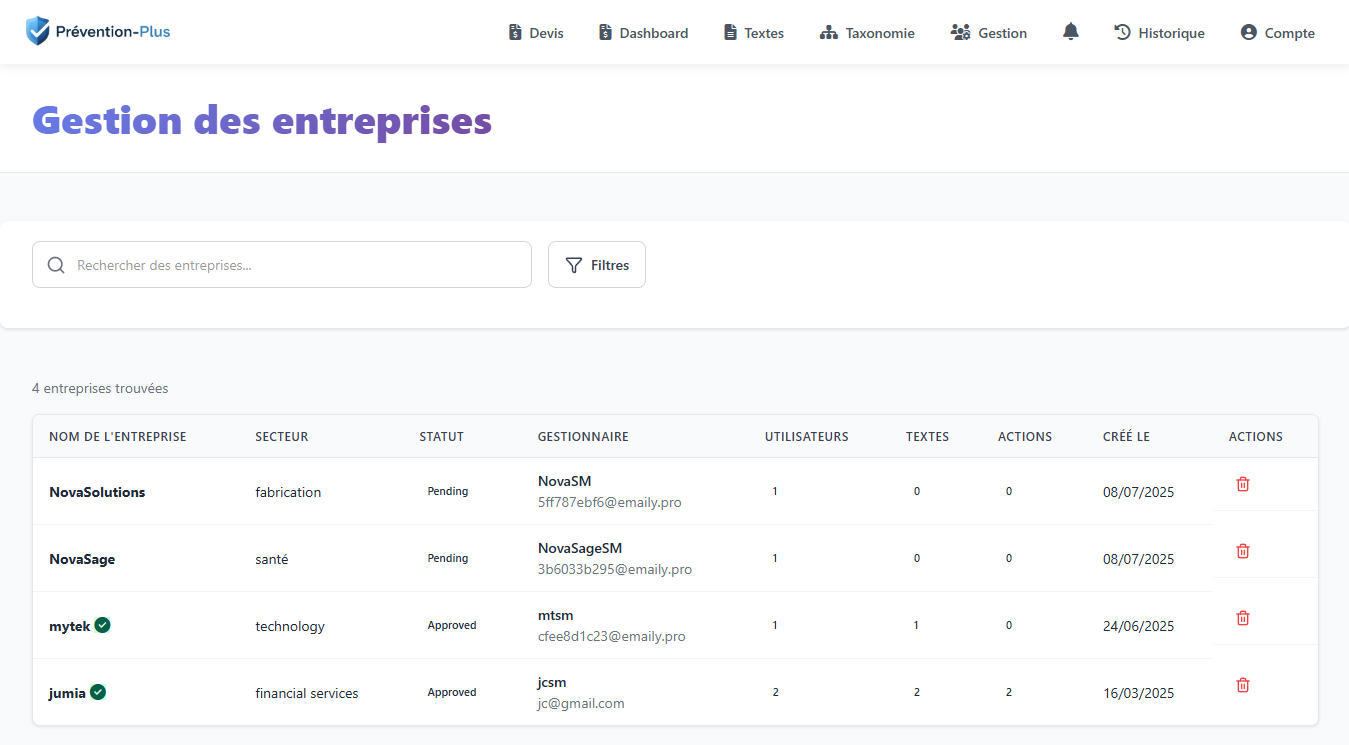
\includegraphics[width=14cm,height=9cm]{images/gestionentreprises.PNG}
    \caption{Interface de gestion des entreprises}
\end{figure}


\subsubsection{Interface des paramètres d'entreprise}
\noindent La figure 4.30 présente l'interface des paramètres d'entreprise permettant à l'Admin de consulter et modifier les informations de son entreprise.

\begin{figure}[H]
    \centering
    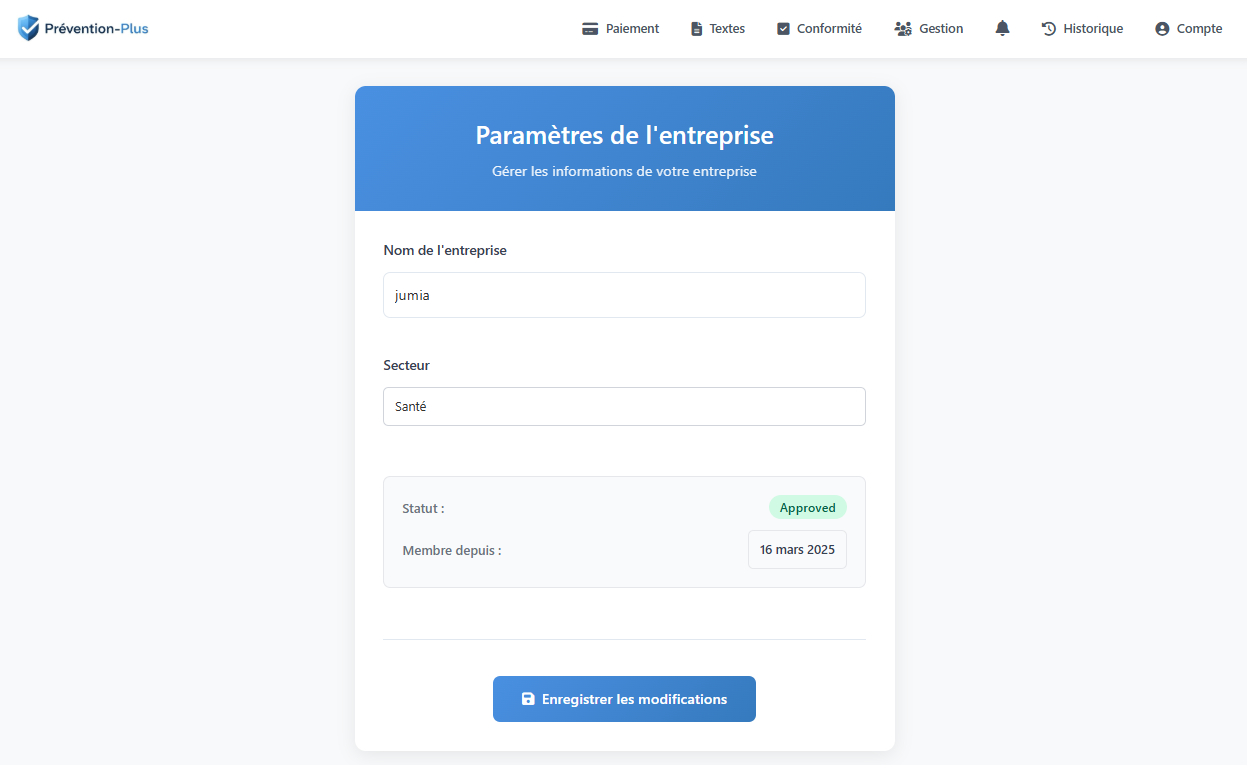
\includegraphics[width=14cm,height=9cm]{images/parametresentreprise.PNG}
    \caption{Interface des paramètres d'entreprise}
\end{figure}

\subsubsection{Interface de gestion de la taxonomie}
\noindent La figure 4.31 présente l'interface de gestion de la taxonomie pour le Super Admin permettant de créer, modifier et supprimer les éléments de taxonomie.

\begin{figure}[H]
    \centering
    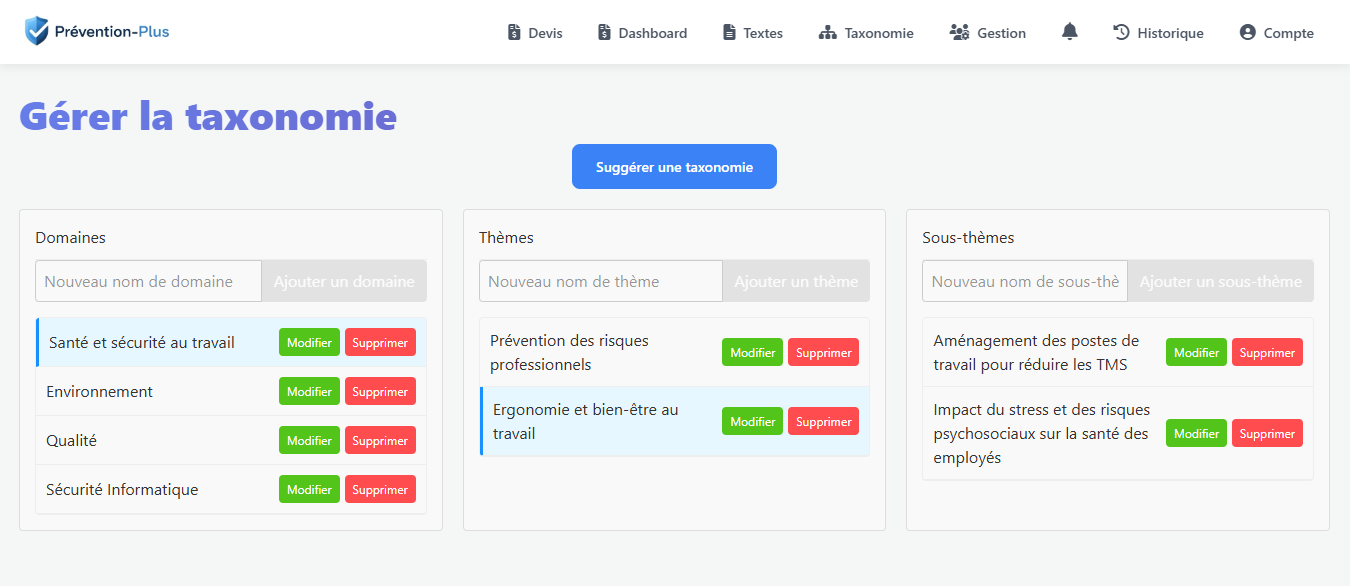
\includegraphics[width=14cm,height=9cm]{images/gestiontaxonomy.PNG}
    \caption{Interface de gestion de la taxonomie}
\end{figure}

\subsubsection{Interface de suggestion de taxonomie par IA}
\noindent La figure 4.32 présente l'interface de suggestion de taxonomie par IA permettant au Super Admin de générer automatiquement des structures de taxonomie.

\begin{figure}[H]
    \centering
    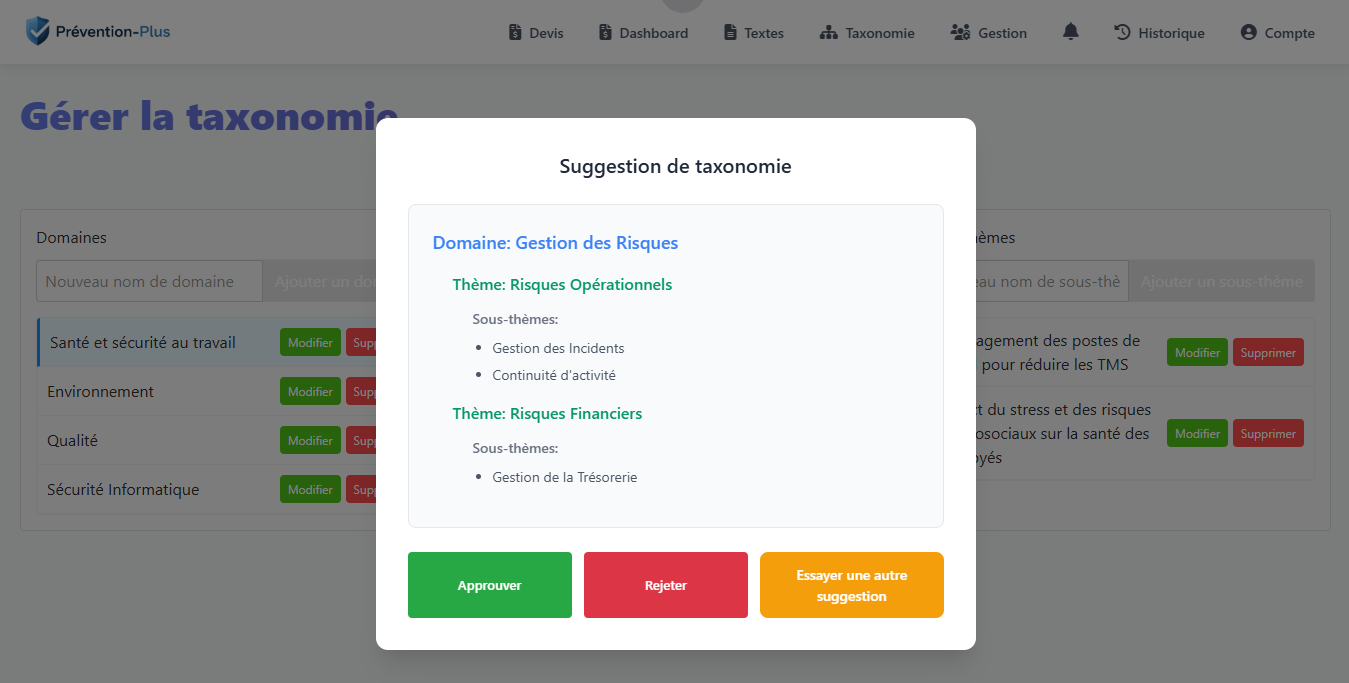
\includegraphics[width=14cm,height=9cm]{images/suggestiontaxonomy.PNG}
    \caption{Interface de suggestion de taxonomie par IA}
\end{figure}

\section*{CONCLUSION}
\noindent Cette première release a permis d'établir les fondations du système « Prévention Plus » avec l'implémentation des fonctionnalités d'authentification, d'inscription, de gestion des profils et de gestion des utilisateurs.
 Le premier sprint a créé les mécanismes d'accès au système, tandis que le second sprint a permis la gestion complète des utilisateurs, entreprises, paramètres d'entreprise et taxonomie tant pour les administrateurs d'entreprise que pour le super administrateur. Ces fonctionnalités constituent la base solide sur laquelle les prochaines releases viendront s'appuyer pour développer les aspects métier de l'application.